% LaTeX Template For MATH 490 @ VCU
\documentclass[11pt]{article}

\usepackage{hyperref}
\usepackage{amsmath}
\usepackage{amsthm}
\usepackage{amssymb}
\usepackage{enumerate}
\usepackage{enumitem}
\usepackage{titlesec}
\usepackage{multicol}
\usepackage{multirow}
\usepackage{mathtools}
\usepackage{mdframed}
\usepackage{tocloft}
\usepackage{tcolorbox}
\usepackage{extarrows}


\setlist{nosep}
\setlist[enumerate]{label=\alph*.}

\renewcommand{\arraystretch}{0.75}

\definecolor{defcolor}{RGB}{255,236,236}    % light red
\definecolor{ngtcolor}{RGB}{255,242,242}    % lighter red
\definecolor{lnkcolor}{RGB}{0,0,180}        % blue
\definecolor{thmcolor}{RGB}{236,236,255}    % light blue
\definecolor{lemcolor}{RGB}{239,239,255}    % lighter blue
\definecolor{procolor}{RGB}{242,242,255}    % lighter lighter blue
\definecolor{crlcolor}{RGB}{245,245,255}    % lighter lighter lighter blue
\definecolor{xmpcolor}{RGB}{255,240,225}    % light orange
\definecolor{rmkcolor}{RGB}{233,255,235}    % light green
\definecolor{axicolor}{RGB}{255,255,233}    % light yellow
\definecolor{notcolor}{RGB}{255,255,244}    % lighter yellow
\definecolor{whacolor}{RGB}{250,250,250}    % lighter gray
\definecolor{reccolor}{RGB}{255,244,255}    % lighter purple

\hypersetup{
    colorlinks,
    citecolor=lnkcolor,
    filecolor=lnkcolor,
    linkcolor=lnkcolor,
    urlcolor=lnkcolor
}

\newtheoremstyle{break}
    {\topsep/1.5} % space above
    {\topsep/2.2} % space below
    {}          % body font
    {}          % indent amount
    {\rmfamily} % theorem head font
    {.}          % punctuation after theorem head
    {0.5em}  % space after theorem head
    {\textbf{\thmname{#1}\thmnumber{ #2}}\thmnote{\text{ (#3)}}}
                % theorem hed spec. (empty = "normal")

\theoremstyle{break}
\newmdtheoremenv{theorem}{Theorem}
\newmdtheoremenv{corollary}[theorem]{Corollary}
\newmdtheoremenv{lemma}[theorem]{Lemma}
\newmdtheoremenv{axiom}[theorem]{Axiom}
\newmdtheoremenv{notation}[theorem]{Notation}
\newmdtheoremenv{definition}[theorem]{Definition}
\newmdtheoremenv{remark}[theorem]{Remark}
\newmdtheoremenv{example}[theorem]{Example}
\newmdtheoremenv{problem}[theorem]{Problem}
\newmdtheoremenv{question}[theorem]{Question}

\DeclareMathOperator{\arcsec}{arcsec}
\DeclareMathOperator{\arccot}{arccot}
\DeclareMathOperator{\arccsc}{arccsc}
\DeclareMathOperator{\interior}{int}
\DeclareMathOperator{\closure}{cl}
\DeclareMathOperator{\boundary}{bd}

\newcommand{\dd}{\text{d}}
\newcommand{\ddi}{\text{$\,$d}}
\newcommand{\qqed}{{\hfill$\blacksquare$}}
\newcommand{\defeq}{\overset{\text{def}}{=}}
\newcommand{\transpose}{\text{T}}

\linespread{1.9}
\setlength{\textwidth}{6.9in}
\setlength{\textheight}{9.2in}
\setlength{\oddsidemargin}{-0.2in}
\setlength{\evensidemargin}{-0.2in}
\setlength{\topmargin}{-0.2in}
\setlength{\headheight}{0in}
\setlength{\headsep}{0in}
\setlength{\footskip}{0.5in}
\setlength{\multicolsep}{6.2pt}
\setlength{\belowdisplayskip}{0pt}
%\setlength{\belowdisplayshortskip}{0pt}
\setlength{\abovedisplayskip}{0pt}
%\setlength{\abovedisplayshortskip}{0pt}

\setcounter{section}{0}
\numberwithin{equation}{theorem}

\makeatletter
\newcommand{\vast}{\bBigg@{4}}
\newcommand{\Vast}{\bBigg@{5}}
\makeatother
\title{Homework 5 of Computational Mathematics}
\author{Chang, Yung-Hsuan\\111652004\\Department of Applied Mathematics}

\begin{document}
\maketitle
\thispagestyle{empty}
\newpage
\pagenumbering{arabic}

\begin{problem}\label{problem 1} % 5.1 2bc
    Show that each of the following initial-value problems has a unique solution and find the solution. Can Theorem 5.4 be applied in each case?
    \begin{enumerate}
        \item $y'=t^{-2}(\sin2t-2ty), \quad 1\leq t\leq 2, \quad y(1)=2$; and
        \item $y'=-y+t\sqrt{y}, \quad 2\leq t\leq 3, \quad y(2)=2$.
    \end{enumerate}
\end{problem}
\textbf{Solution}. 
\begin{enumerate}
    \item The domain of $f(t, y)=\dfrac{\sin 2t-2ty}{t^2}$ is $D=[1, 2]\times\mathbb{R}$. It is clear that $f$ is continuous on $D$. Fix a $t\in[1, 2]$. Then, for $y_1, y_2\in\mathbb{R}$, \begin{align*}
        |f(t, y_1)-f(t, y_2)|&=\dfrac{2t|y_1-y_2|}{t^2}\\
        &\leq2|y_1-y_2|,
    \end{align*}
    which implies $f$ satisfies a Lipschitz condition in the variable $y$ on $D$ with a Lipschitz constant $2$. By Theorem 5.4, the initial-value problem has a unique solution. Using algebra, we have \begin{align*}
        t^2y'+2ty&=\sin 2t\\
        t^2y&=-\dfrac{1}{2}\cos2t+C\\
        \overset{y(1)=2}{\implies}\qquad\qquad\quad\quad y&=\dfrac{-\cos2t+4+\cos2}{2t^2}.
    \end{align*}
    \item 
\end{enumerate}


\newpage
\begin{problem}\label{problem 2} % 5.1 4ab
    For each choice of $f(t, y)$ given in parts (a)-(d):
    \begin{enumerate}[label=\roman*.]
        \item Does $f$ satisfy a Lipschitz condition on $D=\{(t, y)\mid 0\leq t\leq1, -\infty<y<\infty\}$?
        \item Can Theorem 5.6 be used to show that the initial-value problem $$y'=f(t, y),\quad 0\leq t\leq 1, \quad y(0)=1$$ is well-posed?
    \end{enumerate}
    \begin{enumerate}
        \item $f(t, y)=e^{t-y}$; and
        \item $f(t, y)=\dfrac{1+y}{1+t}$.
    \end{enumerate}
\end{problem}
\textbf{Solution}. 
\begin{enumerate}
    \item Fix a $t\in[0, 1]$. Then, for $y_1, y_2\in\mathbb{R}$ with $y_1>y_2$, \begin{align*}
        \left|e^{t-y_1}-e^{t-y_2}\right|&\geq \left|e^{-y_1}-e^{-y_2}\right|\\
        &\geq e^{-y_2}
    \end{align*}
    is unbounded, which implies that $f$ does not satisfy a Lipschitz condition on $D$ in the variable $y$. We cannot use Theorem 5.6 here since $f$ does not satisfy a Lipschitz condition.
    \item Fix a $t\in[0, 1]$. Then, for $y_1, y_2\in\mathbb{R}$, \begin{align*}
        \left|\dfrac{1+y_1}{1+t}-\dfrac{1+y_2}{1+t}\right|&\leq|y_1-y_2|,
    \end{align*}
    which implies $f$ satisfies a Lipschitz condition in the variable $y$ on $D$ with Lipschitz constant $1$. Since $f$ is continuous on $D$, by Theorem 5.6, the initial-value problem is well-posed. \qed
\end{enumerate}


\newpage
\begin{problem}\label{problem 3} % 5.2 6ab
    Use Euler's method to approximate the solutions for each of the following initial-value problems.
    \begin{enumerate}
        \item $y'=\dfrac{2-2ty}{t^2+1}, \quad 0\leq t\leq 1, \quad y(0)=1$ with $h=0.1$; and
        \item $y'=\dfrac{y^2}{1+t}, \quad 1\leq t\leq 2, \quad y(1)=-\dfrac{1}{\ln 2}$ with $h=0.1$.
    \end{enumerate}
    Show that the actual solutions are indeed $y(t)=\dfrac{2t+1}{t^2+1}$ and $y(t)=\dfrac{-1}{\ln(t+1)}$, respectively. Plot the errors between your numerical solutions and the exact solutions. Draw your conclusion regarding to the order of error with respect to the time step $\dd t$.
\end{problem}
\textbf{Solution}. 
\begin{enumerate}
    \item We directly differentiate the function and see whether it is a solution. Let $y(t) = \dfrac{2t+1}{t^2+1}$. It is clear that $y(0) = 1$, and we have \begin{align*}
        y'(t) &= \dfrac{2(t^2+1) - (2t+1)(2t)}{(t^2+1)^2}\\
        &= \dfrac{2}{t^2+1} - \dfrac{2t}{t^2+1}\dfrac{2t+1}{t^2+1}\\
        &= \dfrac{2 - 2ty}{t^2+1}.
    \end{align*} The graph of the approximated solution and the actual solution can be seen below. The graph of error can also be seen below.
    \begin{center}
        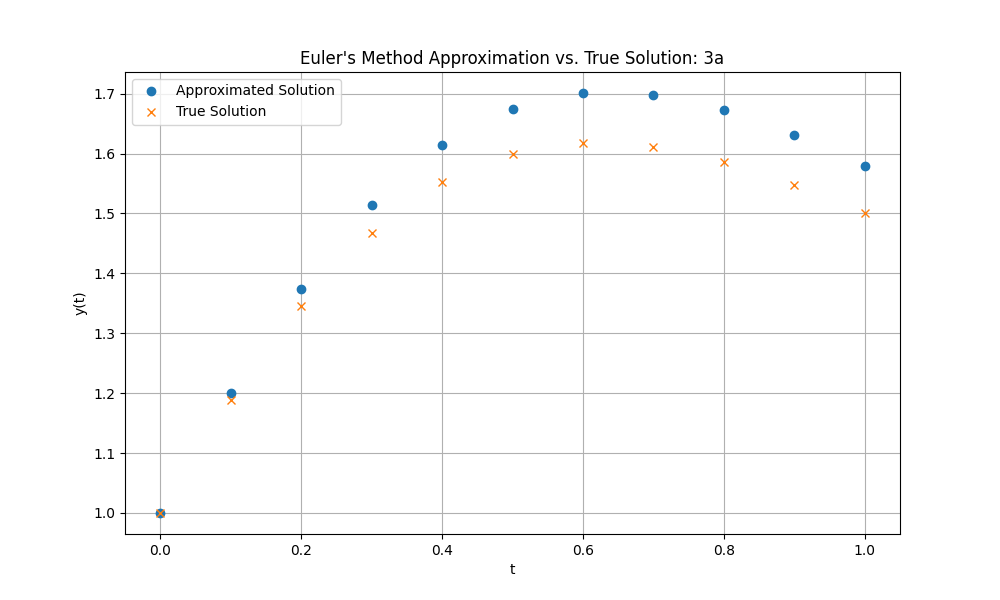
\includegraphics[width=0.7\textwidth]{P3a.png}
    \end{center}
    \begin{center}
        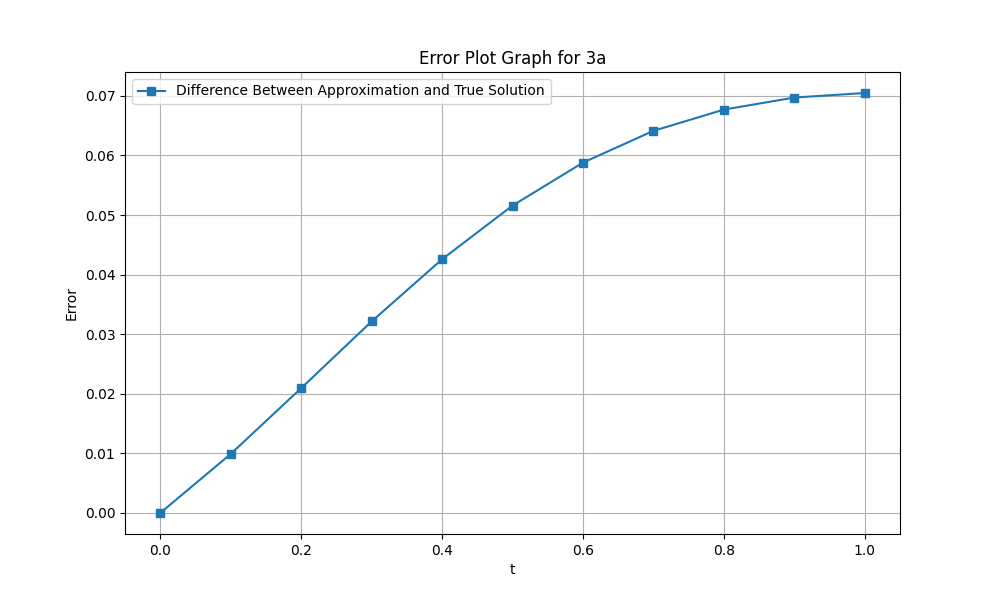
\includegraphics[width=0.7\textwidth]{P3ae.png}
    \end{center}
    \item We directly differentiate the function and see whether it is a solution. Let $y(t) = \dfrac{-1}{\ln(t+1)}$. It is clear that $y(1) = -\dfrac{1}{\ln 2}$, and we have \begin{align*}
        y'(t) &= \dfrac{1/(t+1)}{(\ln(t+1))^2}\\
        &= \dfrac{y^2}{1+t}.
    \end{align*} The graph of the approximated solution and the actual solution can be seen below. The graph of error can also be seen below.
    \begin{center}
        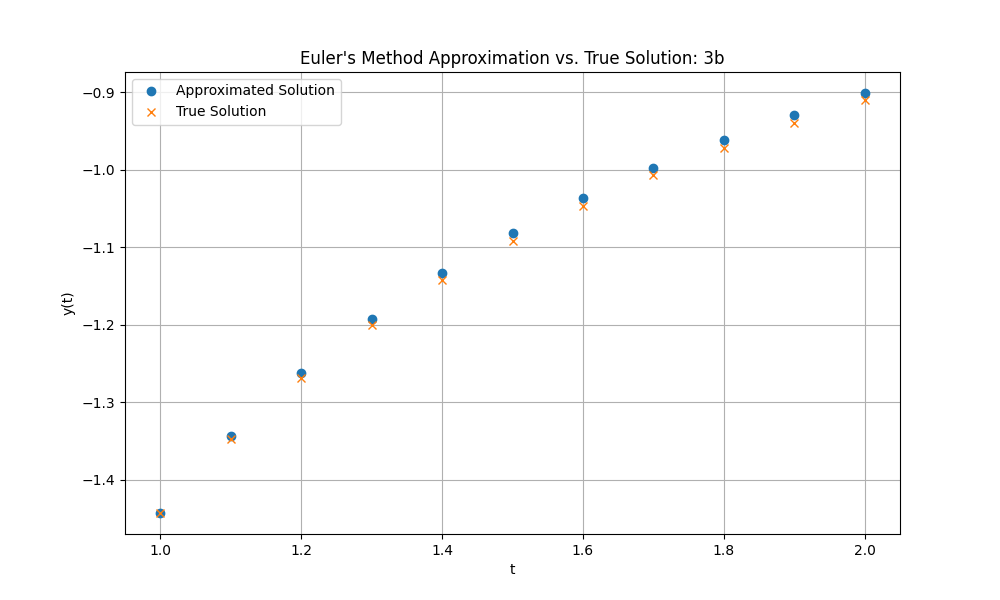
\includegraphics[width=0.7\textwidth]{P3b.png}
    \end{center}
    \begin{center}
        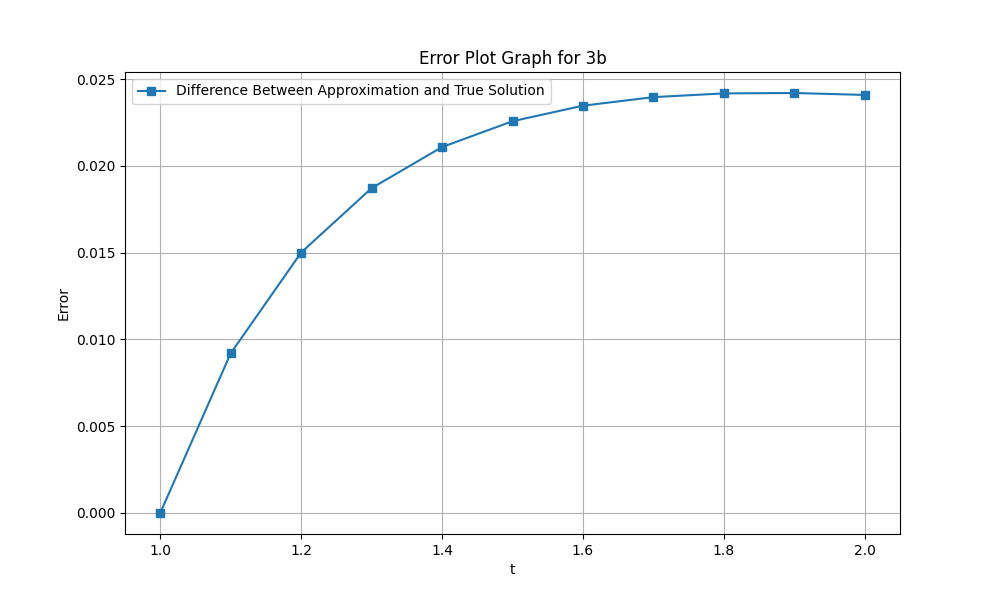
\includegraphics[width=0.7\textwidth]{P3be.png}
    \end{center} \qed
\end{enumerate}


\newpage
\begin{problem}\label{problem 4} % 5.2 11
    Given the initial-value problem $$y'=-y+t+1, \quad 0\leq t\leq 5, \quad y(0)=1$$ with exact solution $y(t)=e^{-t}+t$.
    \begin{enumerate}
        \item Approximate $y(5)$ using Euler's method with $h = 0.2$, $h = 0.1$, and $h = 0.05$.
        \item Determine the optimal value of $h$ to use in computing $y(5)$, assuming $\delta = 10^{-6}$ and that Eq. (5.14) is valid.
    \end{enumerate}
\end{problem}
\textbf{Solution}. 
\begin{enumerate}
    \item Using Euler's method with \begin{equation*}
        \omega_{i+1}=\omega_i+h\:(-y+hi+1), \quad i=1,2,\dots,\dfrac{5-0}{h}.
    \end{equation*}
    By Python, we have \begin{align*}
        y(5)&\approx5.20302231455\quad\text{when $h=0.2$};\\
        y(5)&\approx5.10463839769\quad\text{when $h=0.2$};\\
        y(5)&\approx5.05562450276\quad\text{when $h=0.2$};
    \end{align*}
    \item By assuming (5.14) is true and $\delta=10^{-6}$, the minimal value of $E(h)$ occurs when $$h=\sqrt{\dfrac{2\cdot10^{-6}}{\max_{t\in[0, 5]}|e^{-t}|}}=\sqrt{2\cdot10^{-6}}\approx1.4142135623731\times10^{-3}.$$ \qed
    \begin{center}
        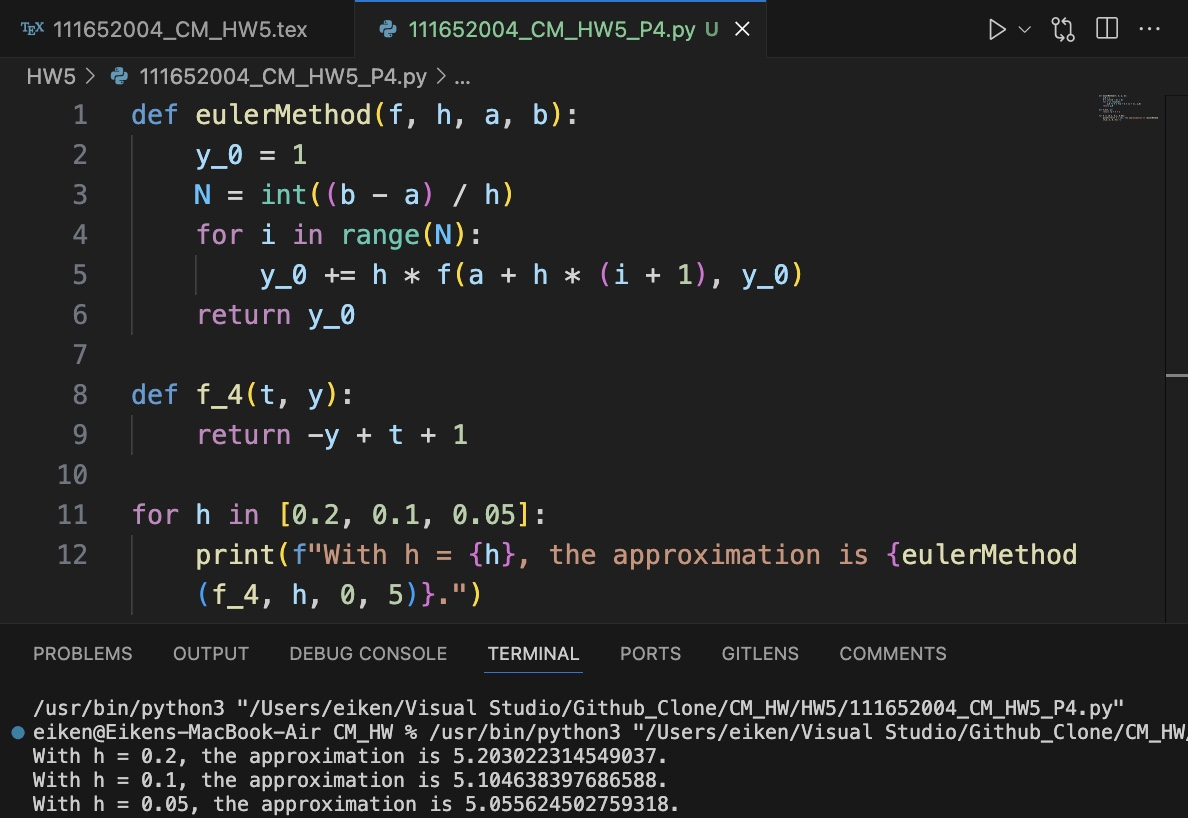
\includegraphics[width=0.7\textwidth]{P4a.jpg}\\
        The code for Problem 4a.
    \end{center}
\end{enumerate}


\newpage
\begin{problem}\label{problem 5} % 5.3 2bc
    Use Taylor's method of order two to approximate the solutions for each of the following initial-value problems.
    \begin{enumerate}
        \item $y'=\dfrac{1+y}{1-t}, \quad 1\leq t\leq 2, \quad y(1)=2$ with $h=0.5$; and
        \item $y'=-y+t\sqrt{y}, \quad 2\leq t\leq 3, \quad y(2)=2$ with $h=0.25$.
    \end{enumerate}
\end{problem}
\textbf{Solution}. 


\newpage
\begin{problem}\label{problem 6} % 5.3 9
    Given the initial-value problem $$y'=\dfrac{2}{t}y+t^2e^t, \quad 1\leq t\leq 2, \quad y(1)=0$$ with exact solution $y(t)=t^2(e^t-e)$.
    \begin{enumerate}
        \item Use Taylor's method of order two with $h = 0.1$ to approximate the solution, and compare it with the actual values of $y$.
        \item Use the answers generated in part (a) and linear interpolation to approximate $y$ at the following values, and compare them to the actual values of $y$.
        \begin{enumerate}[label=\roman*.]
            \item $y(1.04)$;
            \item $y(1.55)$; and
            \item $y(1.97)$.
        \end{enumerate}
        \item Use Taylor's method of order four with $h = 0.1$ to approximate the solution, and compare it with the actual values of $y$.
        \item Use the answers generated in part (c) and piecewise cubic Hermite interpolation to approximate $y$ at the following values, and compare them to the actual values of $y$.
        \begin{enumerate}[label=\roman*.]
            \item $y(1.04)$;
            \item $y(1.55)$; and
            \item $y(1.97)$.
        \end{enumerate}
    \end{enumerate}
\end{problem}
\textbf{Solution}. 


\newpage
\begin{problem}\label{problem 7} % 5.4 4bc
    Use the modified Euler method to approximate the solutions to each of the following initial-value problems, and compare the results to the actual values.\begin{enumerate}
        \item $y'=\dfrac{y^2}{1+t}, \quad 1\leq t\leq 2, \quad y(1)=-\dfrac{1}{\ln 2}$ with $h=0.1$; actual solution $y=\dfrac{-1}{\ln(t+1)}$; and
        \item $y'=\dfrac{y^2+y}{t}, \quad 1\leq t\leq 3, \quad y(1)=-2$ with $h=0.2$; actual solution $y(t)=\dfrac{2t}{1-2t}$.
    \end{enumerate}
\end{problem}
\textbf{Solution}. By Python, we have the following results:
\begin{enumerate}
    \item The first graph is with approximated solution and the actual solution; the second graph is the error plot graph. In the error plot graph, I used lines to connect each pair of adjacent dots to increase visual clarity. \begin{center}
        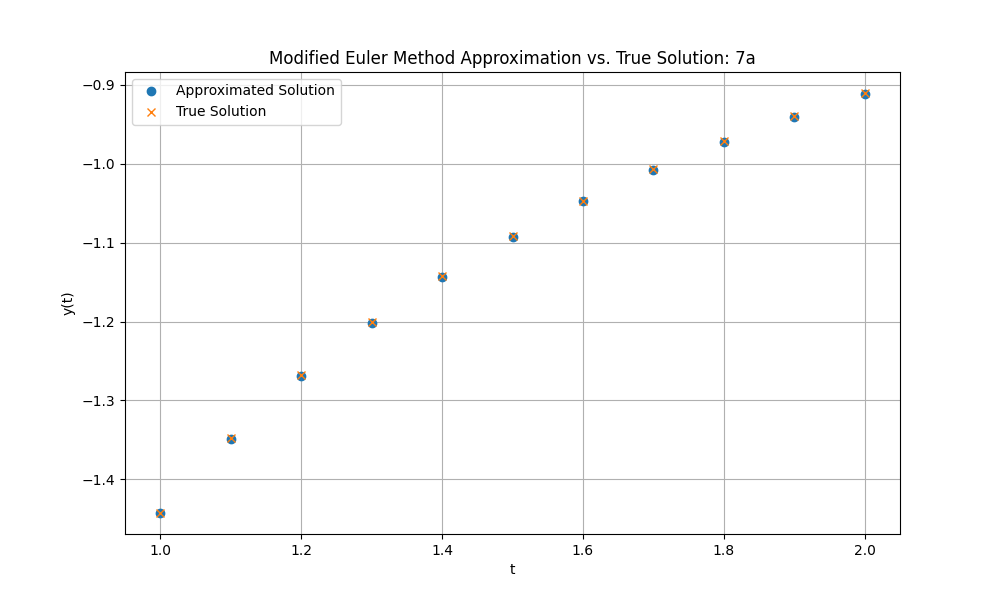
\includegraphics[width=0.7\textwidth]{P7a.png}
    \end{center}
    \begin{center}
        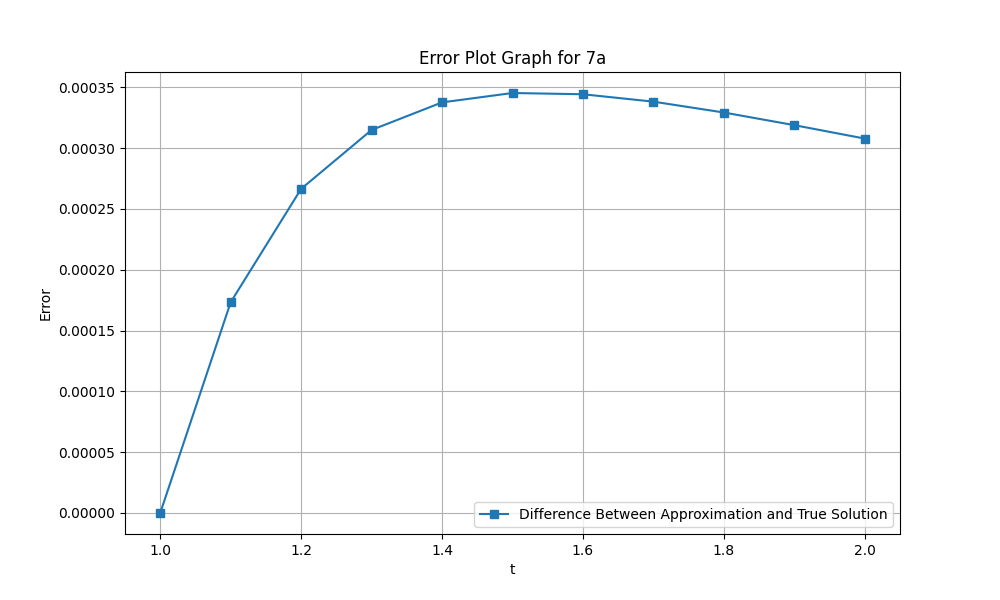
\includegraphics[width=0.7\textwidth]{P7ae.png}
    \end{center}
    \item The first graph is with approximated solution and the actual solution; the second graph is the error plot graph. In the error plot graph, I used lines to connect each pair of adjacent dots to increase visual clarity.
    \begin{center}
        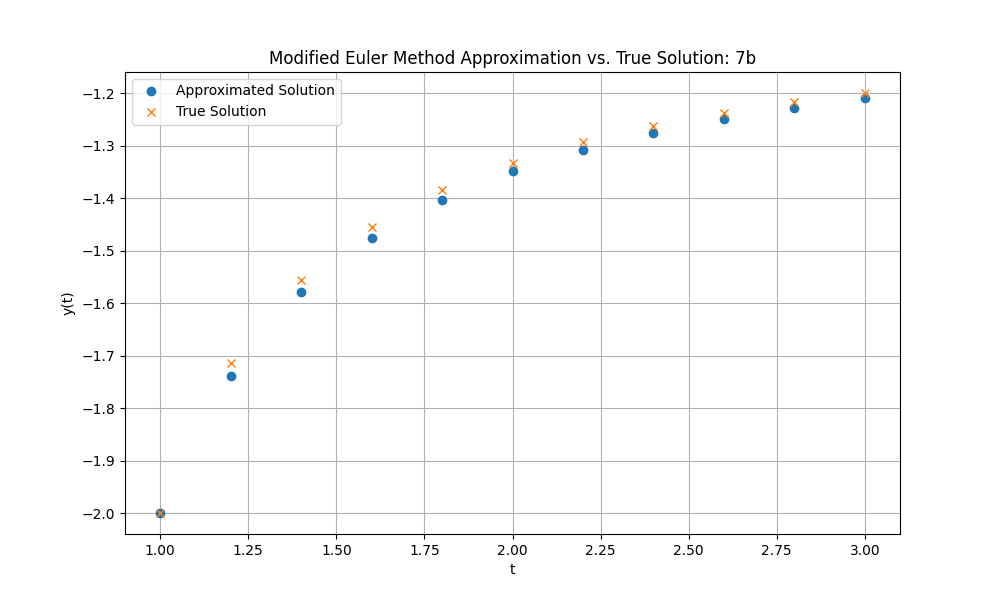
\includegraphics[width=0.7\textwidth]{P7b.png}
    \end{center}
    \begin{center}
        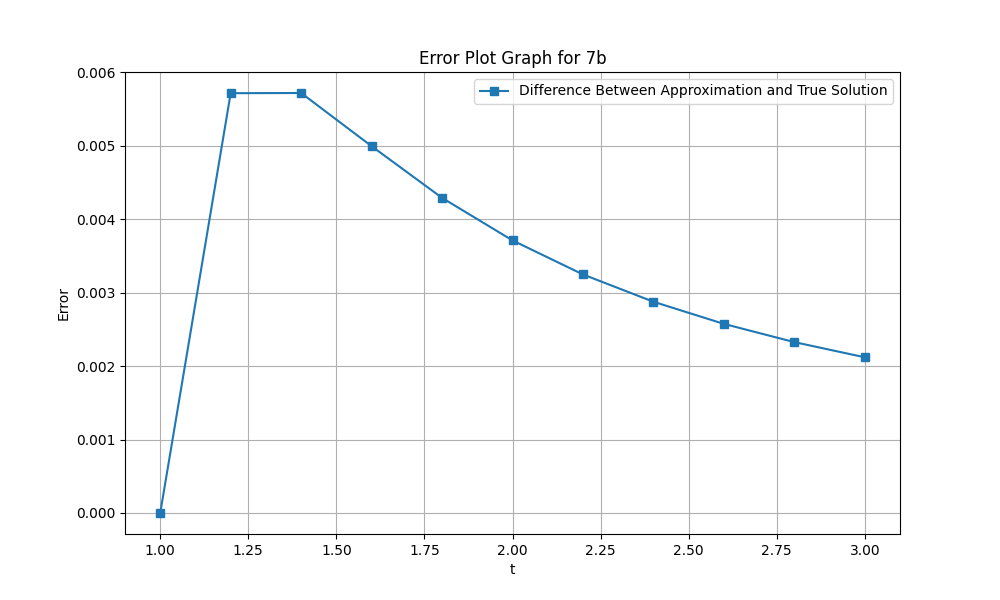
\includegraphics[width=0.7\textwidth]{P7be.png}
    \end{center} \qed
\end{enumerate}


\newpage
\begin{problem}\label{problem 8} % 5.4 30
    Show that the difference method 
    \begin{align*}
        \omega_0&=\alpha\\
        \omega_{i+1}&\omega_i+a_1\:f(t_i, \omega_i)+a_2\:f(t_i+\alpha_2, \omega_1+\delta_2\:f(t_i, \omega_i)),
    \end{align*}
    for each $i=0,1,2,\dots, N-1$, cannot have local truncation error $\mathcal{O}(h^3)$ for any choice of constants $a_1$, $a_2$, $\alpha_2$, and $\delta_2$.
\end{problem}
\textbf{Solution}. 


\newpage
\begin{problem}\label{problem 9} % 5.5 2ab
    Use the Runge-Kutta-Fehlberg algorithm with tolerance $TOL = 10^{-4}$ to approximate the solution to the following initial-value problems.
    \begin{enumerate}
        \item $y'=\left(\dfrac{y}{t}\right)^2+\dfrac{y}{t}, \quad 1\leq t\leq 1.2, \quad y(1)=1$ with $hmax=0.05$ and $hmin=0.02$; and
        \item $y'=\sin t+e^{-t}, \quad 0\leq t\leq 1, \quad y(0)=0$ with $hmax=0.25$ and $hmin=0.02.$
    \end{enumerate}
\end{problem}
\textbf{Solution}. The code is provided after the two graphs.
\begin{enumerate}
    \item $\ $
    \begin{center}
        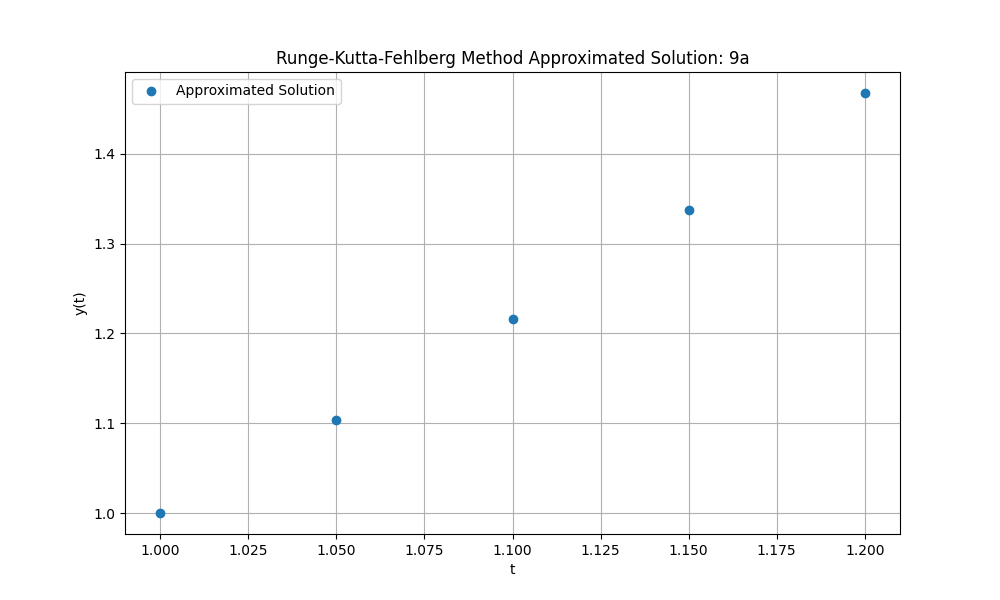
\includegraphics[width=0.7\textwidth]{P9a.png}
    \end{center}
    \item $\ $
    \begin{center}
        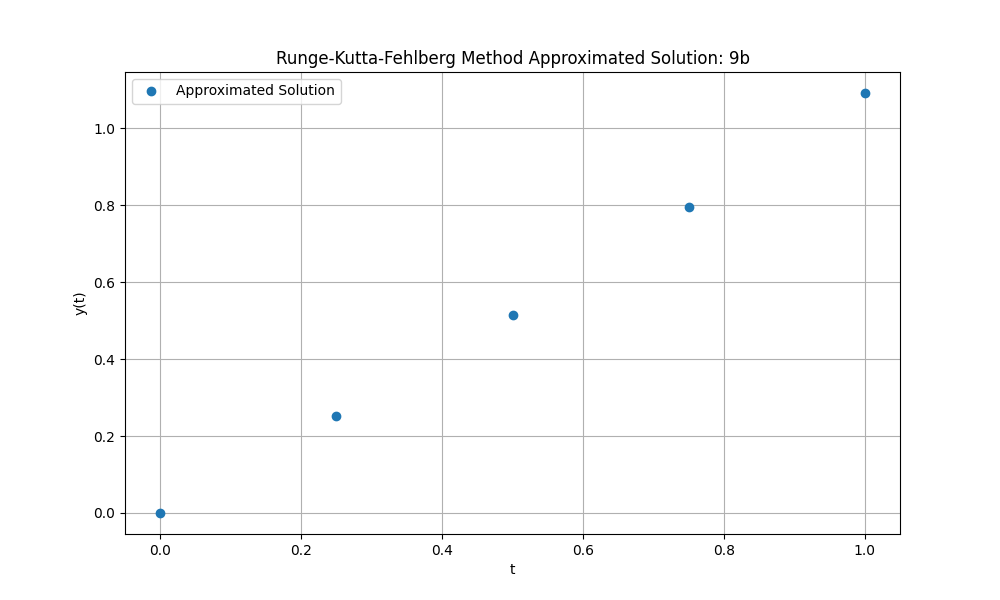
\includegraphics[width=0.7\textwidth]{P9b.png}
    \end{center} \qed
\end{enumerate}

\begin{center}
    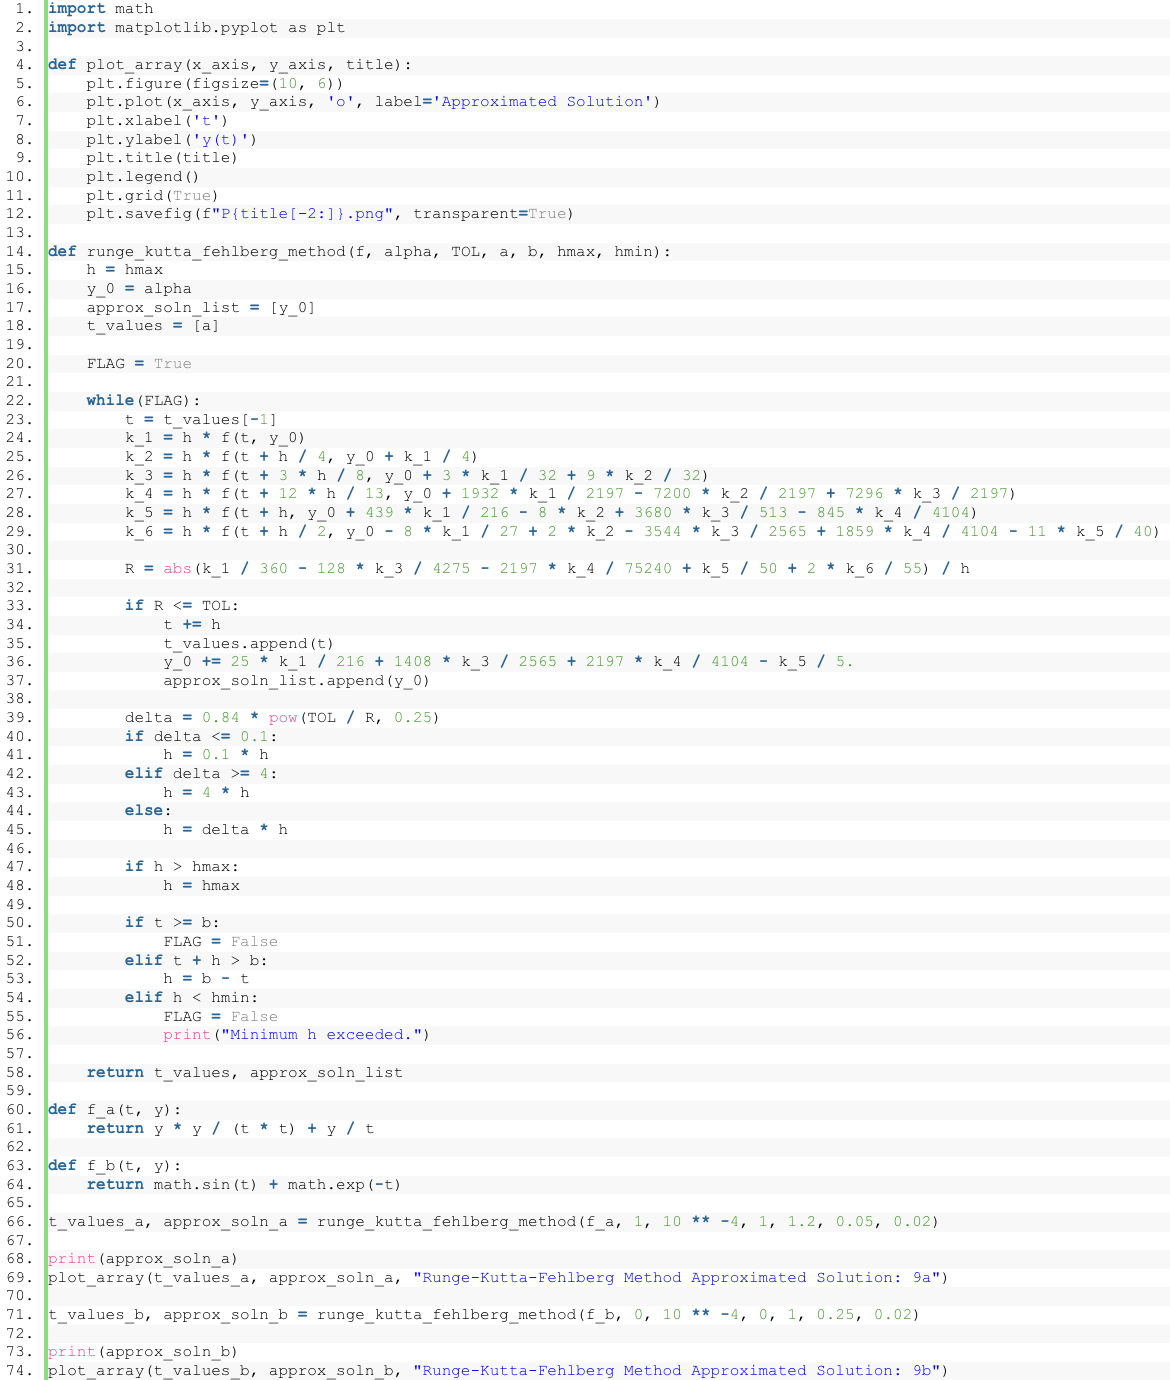
\includegraphics[width=0.9\textwidth]{P9.png}
\end{center}


\newpage
\begin{problem}\label{problem 10} % 5.6 3ad
    Use each of the Adams-Bashforth methods to approximate the solutions to the following initial-value problems. In each case use starting values obtained from the Runge-Kutta method of order four. Compare the results to the actual values.
    \begin{enumerate}
        \item $y'=\dfrac{y}{t}-\left(\dfrac{y}{t}\right)^2, \quad1\leq t\leq 2, \quad y(1)=1$ with $h=0.1$; actual solution $y(t)=\dfrac{t}{1+\ln(t)}$; and
        \item $y'=-5y+5t^2+2t, \quad 0\leq t\leq 1, \quad y(0)=\dfrac{1}{3}$ with $h=0.1$; actual solution $y(t)=t^2+\dfrac{e^{-5t}}{3}$.
    \end{enumerate}
\end{problem}
\textbf{Solution}. The code is provided after the two graphs.
\begin{enumerate}
    \item $\ $
    \begin{center}
        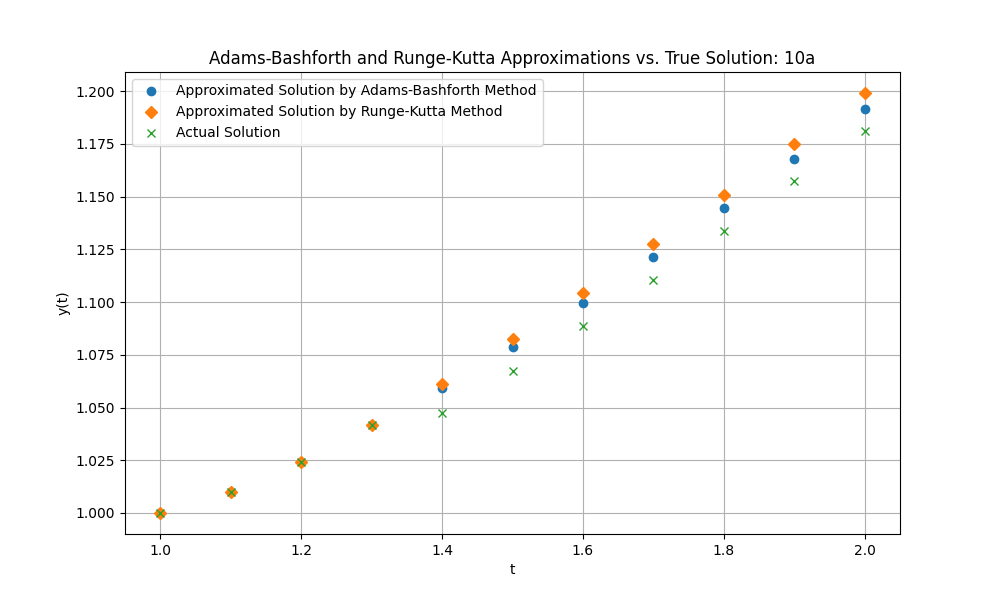
\includegraphics[width=0.7\textwidth]{P10a.png}
    \end{center}
    \item $\ $
    \begin{center}
        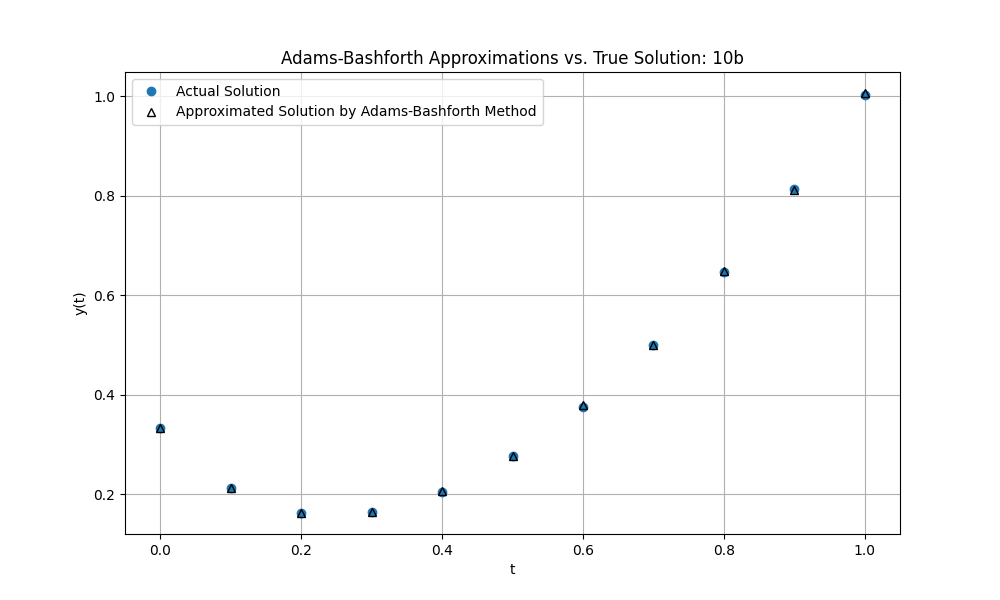
\includegraphics[width=0.7\textwidth]{P10b.png}
    \end{center} \qed
\end{enumerate}

\begin{center}
    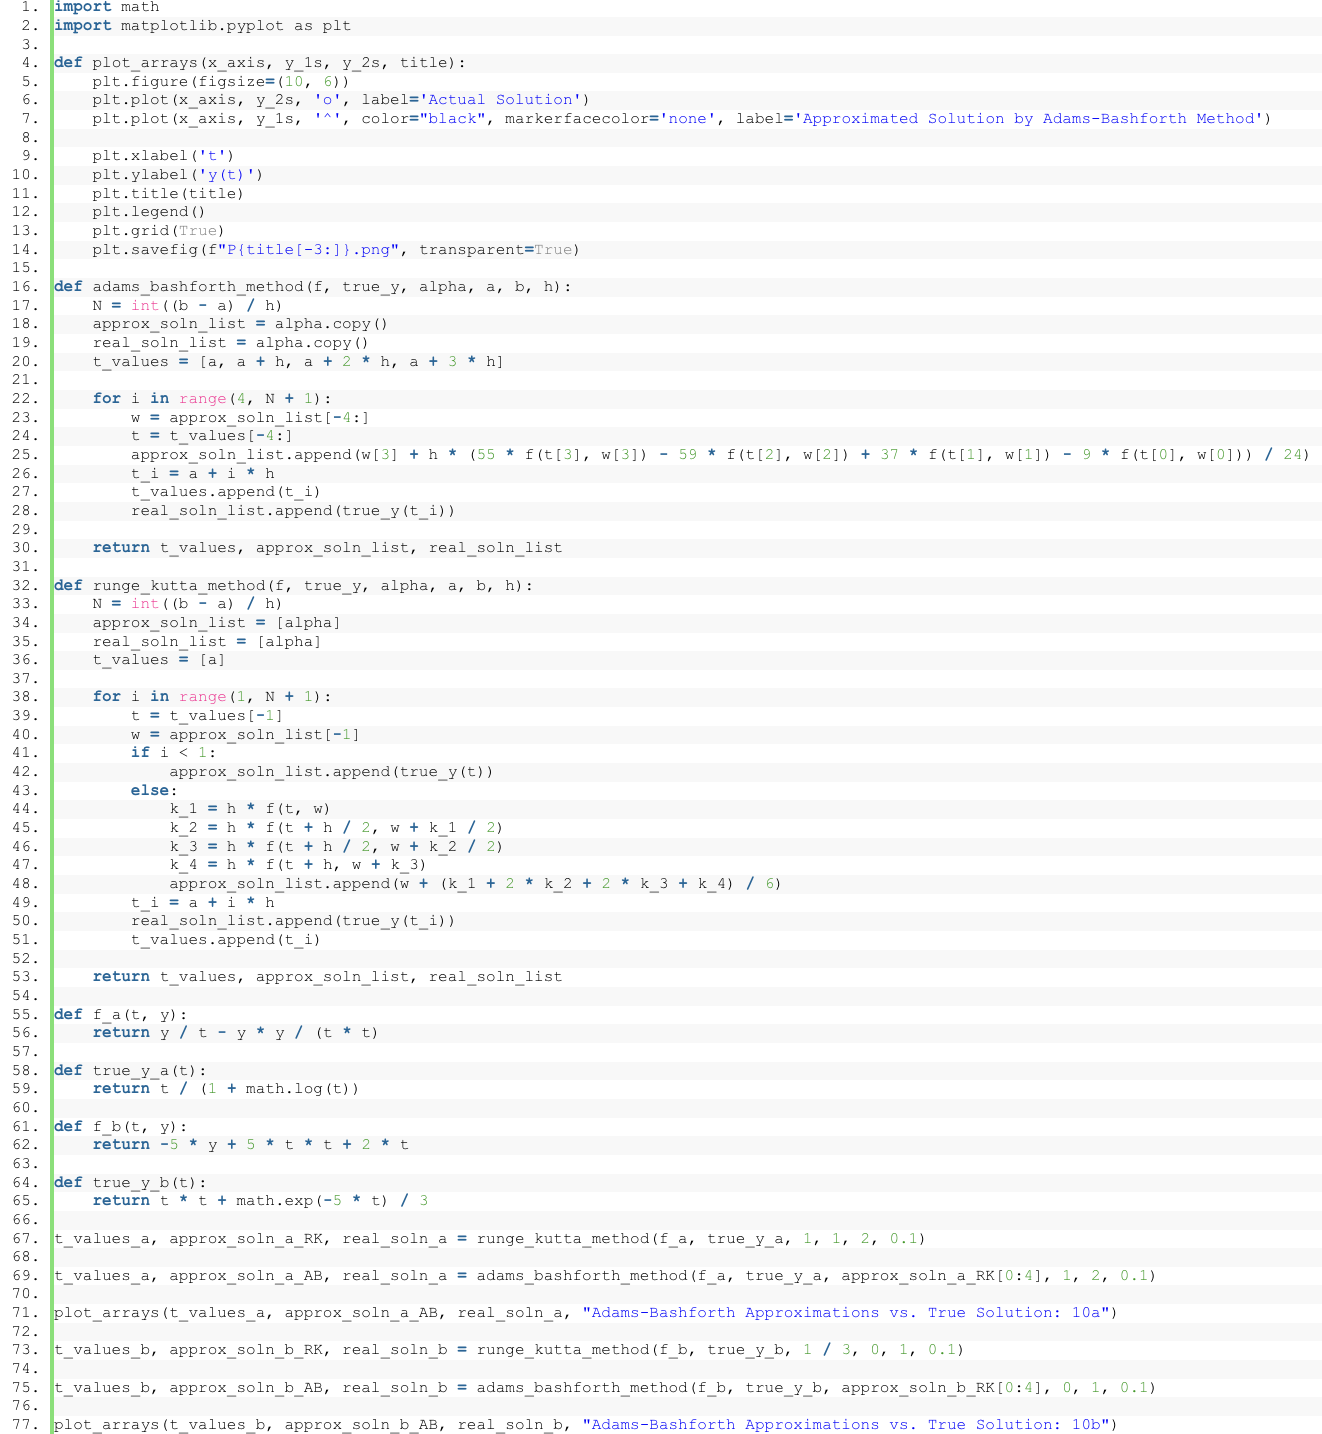
\includegraphics[width=0.9\textwidth]{P10.png}
\end{center}


\newpage
\begin{problem}\label{problem 11} % 5.6 9
    The initial-value problem $$y'=e^y, \quad 0\leq t\leq 0.2, \quad y(0)=1$$ has solution $y(t)=1-\ln(1-et)$. Applying the three-step Adams-Moulton method to this problem is equivalent to finding the fixed point $\omega_{i+1}$ of $$g(\omega)=\omega_i+\dfrac{h}{24}\left(9e^\omega+19e^{\omega_i}-5e^{\omega_{i-1}}+e^{\omega_{i-2}}\right).$$
    \begin{enumerate}
        \item With $h = 0.01$, obtain $\omega_{i+1}$ by functional iteration for $i = 2, \dots , 19$ using exact starting values $\omega_0$, $\omega_1$, and $\omega_2$. At each step use $\omega_i$ to initially approximate $\omega_{i+1}$.
        \item Will Newton's method speed the convergence over functional iteration?
    \end{enumerate}
\end{problem}
\textbf{Solution}. 


\newpage
\begin{problem}\label{problem 12} % 5.6 12
    Derive the Adams-Bashforth three-step method by the following method. Set $$y(t_{i+1})=t(t_i)+ah\:f(t_i, y(t_i))+bh\:f(t_{i-1}, y(t_{i-1}))+ch\:f(t_{i-2}, y(t_{i-2})).$$ Expand $y(t_{i+1})$, $f(t_{i-2}, y(t_{i-2}))$, and $f(t_{i-1}, y(t_{i-1}))$ in Taylor series about $(t_i, y(t_i))$, and equate the coefficients of $h$, $h^2$, and $h^3$ to obtain $a$, $b$, and $c$.
\end{problem}
\textbf{Solution}. 


\newpage
\begin{problem}\label{problem 13} % 5.7 2bd
    Use the Adams variable step-size predictor-corrector algorithm with $TOL = 10^{-4}$ to approximate the solutions to the following initial-value problems:
    \begin{enumerate}
        \item $y'=\sin t+e^{-t}, \quad 0\leq t\leq 1, \quad y(0)=0$ with $hmax=0.2$ and $hmin=0.01$; and
        \item $y'=-ty+\dfrac{4t}{y}, \quad 0\leq t\leq 1, \quad y(0)=1$ with $hmax=0.2$ and $hmin=0.01$.
    \end{enumerate}
\end{problem}
\textbf{Solution}. 


\newpage
\begin{problem}\label{problem 14} % 5.8 4
    Let $P(t)$ be the number of individuals in a population at time $t$, measured in years. If the average birth rate $b$ is constant and the average death rate $d$ is proportional to the size of the population (due to overcrowding), then the growth rate of the population is given by the logistic equation $$\dfrac{\dd P}{\dd t}(t)=b\:P(t)-k(P(t))^2,$$ where $d=k\:P(t)$. Suppose $P(0)=50976$, $b=2.9\times10^{-2}$, and $k=1.4\times 10^{-7}$. Find the population after 5 years using the extrapolation method (based on the Euler method and the midpoint method) with times step $h=0.1$. Justify the order of truncation error from your numerical answers.
\end{problem}
\textbf{Solution}. 


\newpage
\begin{problem}\label{problem 15} % 5.9 8a
    Suppose the swinging pendulum described in the lead example of this chapter is $2$ ft long and that $g = 32.17\ \text{ft}/\text{s}^2$. With $h = 0.1\ \text{s}$, compare the angle $\theta$ obtained for the following two initial-value problems at $t = 0, 1, 2$. $$\dfrac{\dd^2\theta}{\dd t^2}+\dfrac{g}{L}\sin\theta=0, \quad \theta(0)=\dfrac{\pi}{6},\quad \theta'(0)=0.$$ You shall use Adams fourth order predictor-corrector algorithm to obtain your numerical answer.
\end{problem}
\textbf{Solution}. 


\newpage
\begin{problem}\label{problem 16} % 5.10 4
    Consider the differential equation $$y'=f(t, y), \quad a\leq t\leq b, \quad y(a)=\alpha.$$
    \begin{enumerate}
        \item Show that $$y'(t_i)=\dfrac{-3y(t_y)+4y(t_{i+1}-y(t_{i+2}))}{2h}+\dfrac{h^2}{3}y'''(\xi_1)$$ for some $\xi\in(t_i, t_{i+2})$.
        \item Part (a) suggests the difference method $$\omega_{i+2}=4\omega_{i+1}-3\omega_{i}-2h\:f(t_i, \omega_i), \quad\text{for}\ i=0,1,2\dots, N-2.$$ Use this method to solve $$y'-1-y, \quad 0\leq t\leq 1, \quad y(0)=0$$ with $h=0.1$. Use the starting values $\omega_0=0$ and $\omega_1=y(t_1)=1-e^{-0.1}$.
        \item Repeat part (b) with $h=0.01$ and $\omega_1=1-e^{-0.01}$.
        \item Analyze this method for consistency, stability, and convergence.
    \end{enumerate}
\end{problem}
\textbf{Solution}.


\newpage
\begin{problem}\label{problem 17} % 5.10 5
    Given the multistep method $$\omega_{i+1}=-\dfrac{3}{2}\omega_i+3\omega_{i-1}-\dfrac{1}{2}\omega_{i-2}+3g\:f(t_i, \omega_i), \quad \text{for}\ i=2,3,\dots, N-1$$ with starting values $\omega_0$, $\omega_1$, and $\omega_2$:
    \begin{enumerate}
        \item Find the local truncation error.
        \item Comment on consistency, stability, and convergence.
    \end{enumerate}
\end{problem}
\textbf{Solution}.


\newpage
\begin{problem}\label{problem 18} % 5.11 11
    Discuss consistency, stability, and convergence for the implicit trapezoidal method $$\omega_{i+1}=\omega_i+\dfrac{h}{2}\left(f(t_{i+1}, \omega_{i+1})+f(t_i, \omega_i)\right),\quad \text{for}\ i=0,1,2,\dots, N-1$$ with $\omega_0=\alpha$ applied to the differential equation $$y'=f(t, y), \quad a\leq t\leq b, \quad y(a)=\alpha.$$
\end{problem}
\textbf{Solution}.


\newpage
\begin{problem}\label{problem 19} % 5.11 10
    Show that the fourth-order Runge-Kutta method, 
    \begin{align*}
        k_1&=h\:f(t_i, \omega_i),\\
        k_2&=h\:f(t_i+h/2, \omega_i+k_1/2),\\
        k_3&=h\:f(t_i+h/2, \omega_i+k_2/2),\\
        k_4&=h\:f(t_i+h, \omega_i+k_3),\\
        \omega_{i+1}&=\omega_{i}+\dfrac{1}{6}\left(k_1+2k_2+2k_3+k_4\right)
    \end{align*}
    when applied to the differential equation $y'=\lambda y$, can be written in the form $$\omega_{i+1}=\left(1+h\lambda+\dfrac{1}{2}(h\lambda)^2+\dfrac{1}{6}(h\lambda)^3+\dfrac{1}{24}(h\lambda)^4\right)\omega_{i}.$$
\end{problem}
\textbf{Solution}.

\end{document}